\section*{CHAPTER 2: DESIGN AND IMPLEMENTATION}
\addcontentsline{toc}{section}{\numberline{}CHAPTER 2: DESIGN AND IMPLEMENTATION}
\setcounter{section}{2}
\setcounter{subsection}{0}
\setcounter{figure}{0}
\setcounter{table}{0}

In this project, we utilized the power of Python and the convenient jupyter notebook to simulate the 64 QAM OFDM system. A full notebook can be seen in the Appendix.

\subsection{OFDM system architecture}
Figure \ref{diagram} shows a block diagram of our generic OFDM system.

\begin{figure}[htbp]
    \centering
    \documentclass[preview]{standalone}

\usepackage[english]{babel}
\usepackage{amsmath}
\usepackage{amssymb}
\usepackage[f]{esvect}
\usepackage{tikz}

\begin{document}

\usetikzlibrary{positioning}
\tikzset{block/.style={draw,thick,minimum width=1cm,minimum height=1cm,align=center}}
\tikzset{node distance=0.5cm}
\tikzset{double distance=1pt}
\tikzset{>=latex}

\begin{tikzpicture}
    \begin{scope}
        \draw [->] (-0.5,0) node [left] {$\vec{b}$}  -- (0,0) node (SP1) [right,block] {S2P};
        \node (M) [block,right=of SP1] {Mapping};
        \node (IFFT) [block,right=of M] {IFFT};
        \node (PS1) [block,right=of IFFT] {P2S};
        \node (CP) [block,right=of PS1] {Add CP};

        \draw [double,->] (PS1) -- (CP);

        \def\lines{
        \draw \ls ([yshift=3.mm]\from.east) -- ([yshift=3.mm]\to.west);
        \draw \ls ([yshift=1.mm]\from.east) -- ([yshift=1.mm]\to.west);
        \draw \ls ([yshift=-1.mm]\from.east) -- ([yshift=-1.mm]\to.west);
        \draw \ls ([yshift=-3.mm]\from.east) -- ([yshift=-3.mm]\to.west);
        }

        \def\ls{[->]}
        \def\from{SP1} \def\to{M} \lines
        \def\ls{[->,double]}
        \def\from{M} \def\to{IFFT} \lines
        \def\from{IFFT} \def\to{PS1} \lines

        \node (C) [block,below right=of CP] {Channel};

        \node (CP1) [block,below left=of C] {Remove CP};
        \node (SP2) [block,left=of CP1] {S2P};
        \node (FFT) [block,left=of SP2] {FFT};
        \node (EQ) [block,left=of FFT] {Equalize};
        \node (CE) [block,below=of EQ] {Channel\\Estimate};
        \node (Dem) [block,left=of EQ] {Demapping};
        \node (PS2) [block,left=of Dem] {P2S};
        \draw [->] (PS2.west) -- +(-0.5,0) node [left] {$\hat{b}$};

        \def\ls{[<-,double]}
        \def\from{SP2} \def\to{CP1} \lines
        \def\from{FFT} \def\to{SP2} \lines
        \def\from{EQ} \def\to{FFT} \lines
        \def\from{Dem} \def\to{EQ} \lines
        \def\ls{[<-]}
        \def\from{PS2} \def\to{Dem} \lines

        \draw [->,double,thick] (FFT.south) |- (CE.east);
        \draw [->,double,thick] (CE.north) -- (EQ.south);

        \draw [->,double] (CP) -| (C);
        \draw [->,double] (C) |- (CP1);
    \end{scope}
\end{tikzpicture}

\end{document}

    \caption{Block diagram of the OFDM system}
    \label{diagram}
\end{figure}

Principles of operation for each block:
\begin{itemize}
    \item S2P (Serial to Parallel): Converts serial data into parallel data, splitting high-speed bit streams into K lower-speed bit streams, where K is the number of subcarrier waves in the system.
    \item Mapping: QAM modulation to map pairs of bits into complex-valued constellation symbols according to the mapping\_table.
    \item IFFT(Inverse Fast Fourier Transform): Performs a fast implementation of the Inverse Discrete Fourier Transform, transforming signals from the time domain to the frequency domain, creating orthogonal subcarrier waves.
    \item P2S (Parallel to Serial): Converts parallel data back to serial, returning the signal stream to its original continuous form for transmission.
    \item Add CP:  This operation concatenates a copy of the last CP samples of the OFDM time domain signal to the beginning. This way, a cyclic extension is achieved.
    \item Channel: The wireless channel between transmitter and receiver. Here, we use a simple two-tap multipath channel.
    \item Remove CP: Remove `CP` from the received signal.
    \item FFT(Fast Fourier Transform): Transforming signals from the frequency domain to the time domain.
    \item Channel Estimate: Based on pilot signals, the receiver estimates the transmission channel using estimation algorithms.
    \item Equalize: For each subcarrier, the influence of the channel is removed such that we get the clear (only noisy) constellation symbols back.
    \item Demapping: Transform the constellation points to the pairs of bits according to the demapping\_table. The demapping table is simply the inverse mapping of the mapping\_table.
\end{itemize}

\subsection{Configurations and Parameters set up}

\begin{enumerate}
    \item $K = 64$ : The number of subcarriers, describes how many subcarriers are available in the OFDM system.
    \item $CP = K//$4 : The length of the cyclic prefix, denotes the number of samples that are copied from the end of the modulated block to the beginning, to yield a cyclic extension of the block.
    \item $P = 8$ : The number of pilots in the OFDM symbol, describes how many carriers are used to transmit known information (i.e. pilots). Pilots will be used at the receiver to estimate the wireless channel between transmitter and receiver.
    \item $pilotValue = 3+3j$ : The known value each pilot transmits.
    \item $\mu = 6$ :Since we simulating 64QAM transmission, we need to define $\mu = \log_{2} 64$ bits per symbol
    \item $SNRDB = 20$ : Signal-to-Noise Ratio in dB, that should occur at the receiver.
\end{enumerate}

After that, we need to define some index sets that describe which carriers transmit pilots and which carriers contain payload.

\begin{figure}[htbp]
    \centering
    
\includegraphics[width=\linewidth]{../Source/results/carrier_index}
    \caption{The Carriers transmit pilots and which carriers contain payload}
    \label{carrier_index}
\end{figure}

Furthermore, the mapping from groups of 6 bits to a 64QAM constellation symbol shall be defined in mapping table.

\begin{figure}[htbp]
    \centering
    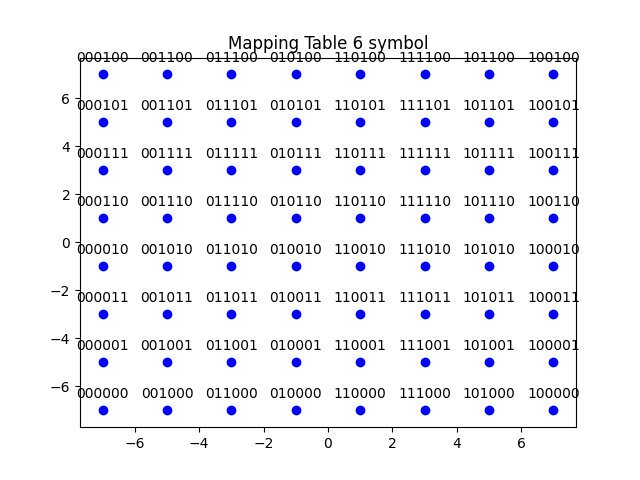
\includegraphics[width=\textwidth]{../Source/results/mapping}
    \caption{64-QAM Constellation with gray-mapping}
    \label{mapping}
\end{figure}

In Figure \ref{mapping}, we have plotted the 64-QAM constellation, along with the bit-labels. In Gray-mapping, two adjacent constellation symbols differ only by one bit and the other 5 bits remain the same. This technique helps to minimize bit-errors, in case a wrong constellation symbol is detected: Most probably, symbol errors are "off-by-one" errors, i.e. a symbol next to the correct symbol is detected. Then, only a single bit-error occurs.

Let us now define the wireless channel between transmitter and receiver. Here, we use a simple two-tap multipath channel with given impulse response channelResponse. Also, we plot the corresponding frequency response. As seen in Figure \ref{channel}, the channel is frequency-selective.

\begin{figure}[htbp]
    \centering
    \includegraphics[width=\textwidth]{../Source/results/channel}
    \caption{64-QAM Constellation with gray-mapping}
    \label{channel}
\end{figure}

\newpage